\documentclass[12pt]{article}
%\usepackage{asd-en}
%\usepackage{templates/ds}
\usepackage{filemod}
\usepackage{caption}
\usepackage{subcaption}
\usepackage[usenames]{color}
\usepackage{graphicx}
\usepackage{amssymb}
\usepackage{amsmath}
\usepackage{amsthm}
\usepackage{url}
\usepackage{times}


\newcommand{\BI}{\begin{itemize}}
\newcommand{\EI}{\end{itemize}}
\newcommand{\BE}{\begin{enumerate}}
\newcommand{\EE}{\end{enumerate}}
\newcommand{\IN}{\mathit{IN}}
\newcommand{\OUT}{\mathit{OUT}}
\newcommand{\receive}{\mathit{receive}}
\newcommand{\send}{\mathit{send}}
\newcommand{\propose}{\mathit{propose}}
\newcommand{\decide}{\mathit{decide}}

\newenvironment{theorem}[1]{\textbf{Theorem (#1)}: }{\medskip}
\newenvironment{lemma}[1]{\textbf{Theorem (#1)}: }{\medskip}

\graphicspath{{figs/06/}}


\begin{document} 

\title{Distributed Systems\\Impossibility of Consensus}
\author{Alberto Montresor\\University of Trento}
\maketitle

\section*{Problem Description}

\BI
\item $n$ processes, each of them {\em proposes} a value;
\item they must {\em decide}, reaching an agreement, one of
  the proposed values.
\EI

\section*{Results}

\BI
\item FLP result: Fischer, Lynch, Paterson~\cite{flp85}: \\
  {\em "Impossibility of Distributed Consensus with one faulty process"} \\
  No algorithms can solve Consensus in an asynchronous distributed
  system in which a single process may crash
  
\item Chandra, Toeug~\cite{ct96} \\
  {\em "Unreliable Failure Detectors for Reliable Distributed Systems} \\
  Introduce the concept of Failure Detector (FD)
  Shows how Consensus can be solved in asynchronous distributed systems
  provided with a FD, even if processes may crash.
\EI

\section*{Some comments}

\BI
\item FLP: Weak consensus specification, strong system model
\item CT: Strong consensus specification, weak system model + FD
\EI
The difference is given by the FD.

\section*{Motivation}

Reaching an agreement on some decision is {\bf the} problem in distributed
computing; consider for example the election of a leader or coordinator, the
agreement on a replicated sensor, etc.

Several problems can be treated like a Consensus problem: Atomic Broadcast, 
Atomic Committment, Group Membership.

\section*{Challenges}

Reaching an agreement in a system without failures is easy. 
On the other hand, reaching an agreement in a system with failures is
more difficult.

Considering different levels of failure models:
\BI
\item Crash
\item Byzantine failures
\item Omission failures
\EI
We can show that even in the simplest of the models, the problem is
not solvable.

\section*{Specification}

\paragraph{Basics}
\BI
\item Set $\Pi = \{ p_1, \ldots, p_n \}$
\item Each process $p_i$ executes $\propose(v_i)$ proposing a value $v_i$
\item Each process $p$ can execute an action $\decide(v)$ in which value
  $v$ is decided.
\item The set of possible values is just $\{ 0, 1\}$.
\EI

\paragraph{(Uniform) Consensus}
\BI
\item {\bf Termination}: Eventually, each correct process decides for some
  value.
\item {\bf (Uniform) Agreement}: All correct processes (all processes) that 
  decide, decide for the same value.
\item {\bf Uniform Validity}
  If a process decides $v$, then $v$ has been proposed by some process.
\item {\bf Uniform Integrity}
  Each process decides at most once.
\EI

\section*{System model}

\BI
\item Asynchronous distributed system 
  \BI
  \item No upper bound to message delays
  \item No upper bound to relative process speeds
  \item No synchronous clocks
  \EI
\item All processes know the $\Pi$ set.
\item No communication failures
\item At most one crash failure, with the crashed process
  stopping executing actions
\EI

\section*{Examples of bad protocols}

\BI
\item All processes decide 0
\item All processes decide 1
\item All processes decide their own value
\item Since $\Pi$ is known, all processes elect deterministically
  the process $p_1$ and wait for a decision from it;
\item Everybody performs a reliable broadcast to everybody; if they receive one zero,
  they decide for 0; otherwise, if they receive all ones, they decide for 1.
\item Majority: everybody decide for the majority it receives
\EI

\section*{Processes, the formal way}

\BI
\item A process $p_i$ is an ``infinite deterministic automata''
\item The {\bf internal state $\sigma_i$} of a process $p_i$ is given by
  the following two registers: 
  \BI
  \item $\IN_i \in \{ 0, 1 \}$: proposed value
  \item $\OUT_i \in \{ 0, 1, \bot \}$: decided value
  \EI
\item Some internal states are {\bf initial states}; if a state $\sigma_i$
  is initial, then $\OUT_i = \bot$.
\item A {\bf decision state} is a state in which $\OUT_i = 0$ or $\OUT_i = 1$.
\item $OUT_i$ is {\em write-once} (uniform integrity)
\EI

\section*{Communication, the formal way}

\BI
\item Message buffer $B$: the set of all sent messages not yet delivered
\item Messages: $\langle p, m \rangle$, where $p$ is the destination, $m$
  is the message from a fixed universe $M$
\item $\send_p(q,m) \Rightarrow B \gets B \cup \{ (q,m) \}$
\item $r=\receive_p()$, there are two cases (chosen in a {\bf non-deterministic} way)
  \BI
    \item If $(p,m) \in B$, then $r=m$ and $B \gets B - \{ (p,m) \}$
    \item or $r = \bot$ (here, means empty message) and the buffer is not
      altered
  \EI
\item \textbf{Perfect channels}:
  $receive()$ may return $\bot$ a finite number of times. But:

  If $p$ executes $receive()$ an infinite number of times, each
  pair $(p,m)$ that is included in $B$ will eventually be received.
\EI

\section*{Configurations, events, schedules, etc.}

\BI
\item {\bf Configuration $C$}: global state consisting of the internal state $\sigma_i$ of each 
  process in $\Pi$ and the content of the message buffer $B$;
\item {\bf Initial configuration}: a configuration in which each state is
  an initial state and the message buffer is empty;
\item {\bf Event}:
  An event $e = (p_i, m)$ brings the system from a configuration $C$ to another one 
  and consists of a primitive step of a single process $p_i$.
  \BI
  \item $m = \receive_i()$; $p_i$ receives a message from the message buffer of $C$; \\
    $m \in M \cup \{ \bot \}$ and $(p,m) \in B$.
  \item Based on $\sigma_i$ and $m$, $p$ enters in a new state
  \item $p_i$ may send a finite set of messages to other processes
  \EI
\item Given an event $e$ and a configuration $C$, then:
  \BI
  \item $C' = e(C)$ is the {\bf resulting configuration} of $e$ and $C$;
  \item We say that $e$ can be {\bf applied} to $C$
  \EI
\item Given a configuration $C$, we say that a sequence of events $s=e_1 e_2 \ldots e_k$ is 
  a {\bf schedule} that can be {\bf applied} from $C$ if 
  \[
    C' = e_k(e_{k-1}(\ldots(e_2(e_1(C)))\ldots))
  \]
\item We say that a configuration has a {\bf decision value} $v$ if:
  $\exists p_i \in \Pi: \OUT_i = v$.
\item A {\bf run} is an infinite schedule that can be applied to an initial configuration.
\item {\bf Admissible run}: a run in which:
  \BI
  \item At most one process is faulty;
  \item Eventually, all messages sent to correct processes are delivered
  \EI
\item {\bf Deciding run}: a run in which there is a configuration with 
  a decision value.
\EI

\section*{Pros and Cons}

\paragraph{Positive aspects (powerful system)}
\BI
\item Infinite state automata
\item Reliable communication and broadcast
\item Max 1 failure
\item Set $\Pi$ known to everybody
\item Simple problem: we only consider Consensus
\EI

\paragraph*{Negative aspects (bad environment)}
\BI
\item Asynchronous system
\EI

\section*{The main theorem}

\begin{theorem}{Impossibility}
No Consensus protocol is totally correct if a single crash is possible.
\end{theorem}

\begin{proof}
We prove the theorem by contradiction: we assume that a totally correct 
protocol $P$ exists, and we derive a contradiction.

Let $C$ a configuration and let $V(C)$ the set of decision values in
the decision configurations reachable from $C$:
\BI
\item If $V(C) = \{ 0 \}$, $C$ is {\bf 0-valent}, {\bf univalent}
\item If $V(C) = \{ 1 \}$, $C$ is {\bf 1-valent}, {\bf univalent}
\item If $V(C) = \{ 0,1 \}$, $C$ is {\bf bivalent}.
\item If $V(C) = \emptyset$, not possible ($P$ is totally correct).
\EI

\paragraph{Proof plan}

\BE
\item We prove that $P$ has a initial bivalent configuration
\item We prove that is always possible to go from a bivalent configuration to 
  a bivalent configuration
\EE
Thus, given a totally correct protocol $P$, it is always possible to 
create an infinite run completely composed by bivalent configuration
(i.e., in which a decision is never made).

\end{proof}


\begin{lemma}{Schedule Commutativity}	
Assume that from configuration $C$ the schedules
$s_1$ and $s_2$ bring to configurations $C_1$ and $C_2$,
respectively. If the sets of processes that execute actions in
$s_1$ and $s_2$ are disjoint, then $s_1$ can be applied to $C_2$
and $s_2$ can be applied to $C_1$ and both lead to the same configuration
$D$.
\[
  \{ p_i ~|~ (p_i, m) \in s_1 \} \cap \{ p_i ~|~ (p_i, m) \in s_2 \} = \emptyset \Rightarrow s_2(C_1) = D = s_1(C_2)
\]
\end{lemma}

\begin{proof}
It follows from the definition of applicability, as $s_1$ and $s_2$ do not
interact.
\end{proof}

\begin{figure}
\begin{center}
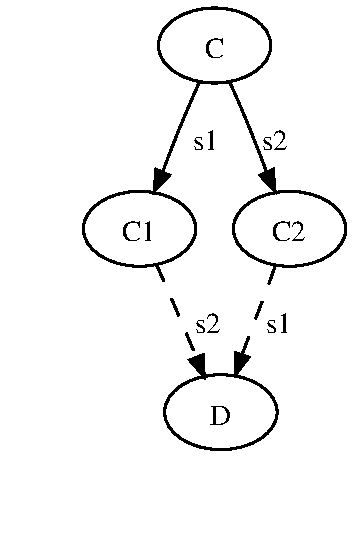
\includegraphics{consensus-fig1.pdf}
\end{center}
\caption{Lemma 1}
\end{figure}


\newpage
\begin{lemma}{Bivalent Initial Configuration}
$P$ has a bivalent initial configuration. 
%
Informally, it means that for some initial
states, the final decision is not deterministically decided by 
the value of the proposed values, but it depends on the order
in which messages are received.
\end{lemma}


\begin{proof}
By contradiction, let us assume that $P$ does not have initial
bivalent configurations.

\BI
\item All configuration are either 0-valent or 1-valent

\item
Each initial configuration could be described by a binary string of proposed
values, such as $1000\ldots0$.

\item 
$P$ must have both 0-valent and 1-valent initial configurations ($00\ldots00$ and
$11\ldots11$); if not, validity would be violated.


\item 
A pair of initial configurations are said {\bf adjacent} if their strings differ
by a single bit. Example: $1000$ and $1100$.

\item
Each pair of initial configuration is linked by a chain of initial configurations, each adjacent
to the following. Example $1000$ -- $1100$ -- $1110$ -- $1111$.

\item Let us consider a chain of initial configuration, where the first is 
  0-valent and the last is 1-valent. In this chain, there should be
  two initial configurations adjacent to each other, one 0-valent ($C_0$) and 
  the other 1-valent ($C_1$).

\item Let $p_i$ be the process whose proposed value differs in the
  two configurations.

\item Let $R$ be an admissible, deciding run from $C_0$ in which
  $p_i$ never executes steps (it is faulty), and let $s$ the associated
  schedule.
\item $s$ can be applied also to $C_1$
\item $s(C_0)$, $s(C_1)$ differ only for the initial value of $p_0$,
  which is faulty; 
\item so the decision in $s(C_1)$ is equal to $s(C_0)$
\item if this decision is 1, in reality $C_0$ is bivalent.
\item if this decision is 0, in reality $C_1$ is bivalent.
\item In both cases, we obtained a contradiction.
\EI
\end{proof}

\newpage

\begin{lemma}{Bivalent-to-Bivalent}~
\BI
\item Let $C$ be a bivalent configuration
\item Let $e=(p_i,m)$ be an event applicable to $C$
\item Let $\hat{C} = \{ s(C) ~|~ e \not\in s \}$ be the set of configuration reachable from $C$ without applying $e$;
\item Let $\hat{D} = e(\hat{C}) = \{ e(C') ~|~ C' \in \hat{C} \}$ be the set of configuration reachable from the configuration
  of $\hat{C}$ by applying $e$.
\EI
Then $\hat{D}$ contains a bivalent configuration.
\end{lemma}

\begin{proof}
By contradiction; $\hat{D}$ does not contain bivalent configurations.

\paragraph{Part 1}
First, we prove that $\hat{D}$ contains both 0-valent and 1-valent configuration. We know that:
\BI
\item $\hat{D}$ does not contain bivalent configuration (by contradiction)
\item $e$ is applicable to $C$ implies that $e$ is applicable to each $E \in \hat{C}$
\item Let $E_i$ be a $i$-valent configuration reachable from $C$ ($i=0,1$); $E_i$ exists
  because $C$ is bivalent;
\EI
The situation can be depicted in this way:
\[
  \text{(0-valent)} \qquad E_0 \xleftarrow{s_0} C \xrightarrow{s_1} E_1 \qquad \text{(1-valent)}
\]

There are two possibilities:
\BI
\item {\bf 1st case}:  
$E_i \in \hat{C}$; the situation can be depicted like this:
\[
  C \xrightarrow{s_i} E_i \xrightarrow{e} F_i
\]
where $E_i$, $F_i$ are $i$-valent, $E_i \in \hat{C}$, $F_i \in \hat{D}$.

\item {\bf 2nd case}:
$E_i \not\in \hat{C}$; the situation can be depicted like this:
\[
  \underbrace{ C \rightarrow \bullet \xrightarrow{e} F_i \rightarrow E_i}_{s_i}
\]
where $E_i$ is $i$-valent; $F_i$ is not bivalent, is not $(1-i)$-valent, so it is
$i$-valent. $F_i \in \hat{D}$.
\EI 

\newpage

\subsubsection*{Part 2}
We want to prove that:
  There exists two configurations $C_0, C_1 \in \hat{C}$ where $C_1=e'(C_0)$ such that
  $e(C_i)=D_i$ is $i$-valent and $D_i \in \hat{D}$.

In the paper: ``easy induction''

There are two cases: $e(C) \in \hat{D}$ can be 0-valent or 1-valent.
Let assume that $e(C)$ is 0-valent (the other case is symmetrical).

Let $s$ be a schedule such that:
\BI
\item $s(C) \in \hat{C}$ (means: $e \not\in s$)
\item $e(s(C))$ is 1-valent (based on Part 1, there is one)
\item $s=e_1 e_2 \ldots e_n$.
\EI

\begin{tabular}{ll}
$e(C)$					& 0-valent, $\in \hat{D}$ \\
$e(e_1(C))$				& 0-valent, $\in \hat{D}$ \\
$D_0=e(e_2(e_1(C))) = e(C_0)$		& 0-valent, $\in \hat{D}$ \\
$D_1=e(e_3(e_2(e_1(C)))) = e(C_1)$	& 1-valent, $\in \hat{D}$ \\
$\ldots$				& 1-valent, $\in \hat{D}$ \\
$e(s(C))$				& 1-valent, $\in \hat{D}$ \\
\end{tabular}
~\\

In other words, we have found $C_0$ and $C_1$ of the claim.

\newpage
\subsubsection*{Part 3}

Let $C_0, C_1=e'(C_0)$ where $e'=(p_j,m')$; we know that
$C_0, C_1 \in \hat{C}$; $D_i = e(C_i)$ is $i$-valent.
%
There are two possibilities:
\BI
\item $p_i \neq p_j$; it is possible to apply Lemma 1, and we obtain
  the diamond of Figure. This is a contradiction, because
  any successor of a 0-valent configuration is 0-valent.
\begin{figure}
\begin{subfigure}[b]{0.30\textwidth}
\begin{center}
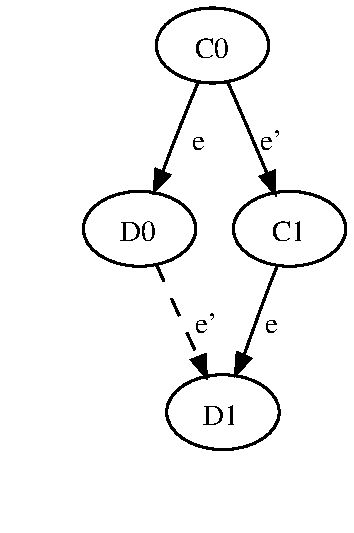
\includegraphics[width=0.95\textwidth]{consensus-fig2.pdf}
\end{center}
\caption{$p_i \neq p_j$}
\end{subfigure}
\begin{subfigure}[b]{0.70\textwidth}
\begin{center}
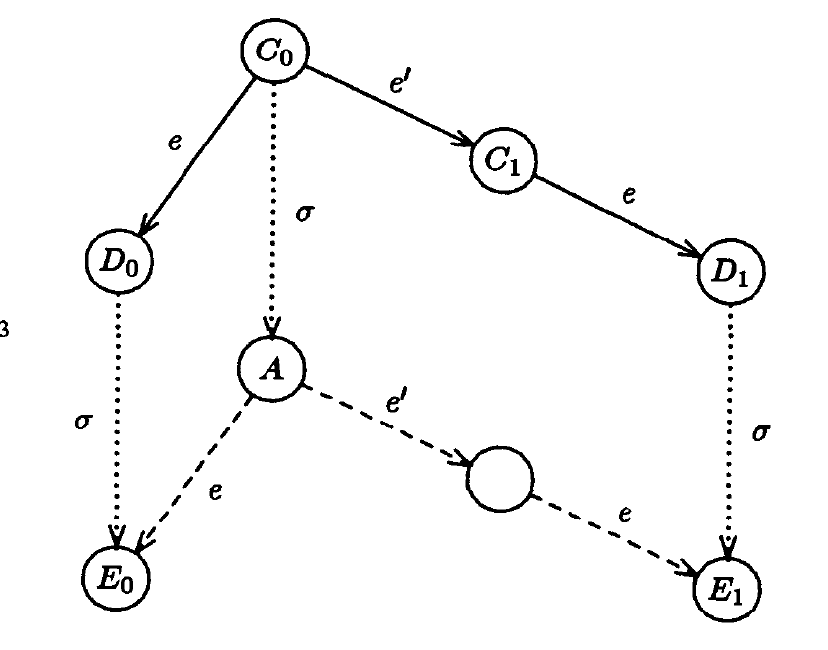
\includegraphics[width=0.95\textwidth]{consensus-fig3.png}
\end{center}
\caption{$p_i = p_j$}
\end{subfigure}
\caption{Lemma 2 - Part 3}
\end{figure}


\item $p_i = p_j$. Let $\sigma$ be a deciding schedule in which $p_i$ never
  executes any event (for example, because it becomes faulty); such schedule
  exists because of total correctness.
  
  From Lemma 1, $\sigma$ is applicable to $D_0$ and $D_1$. But this is a
  contradiction, because from $A$ we can reach both $D_0$ and $D_1$,
  which are $0$-valent and $1$-valent; so $A$ is bivalent, but this
  is impossible, because $\sigma$ is a deciding run.

\EI

\begin{figure}
\end{figure}

What does it mean? That given a bivalent configuration, any decision based on the
observation that a given process $p_i$ is crashed, can be contradicted
by a later action of process $p_i$.

\newpage
\paragraph{Conclusion}

We prove now that given a totally correct protocol $P$, it is always possible 
to build an admissible run which is not deciding; a contradiction.

We cannot ``crash'' more than one process; which means that the other
processes must execute an infinite number of actions.

Elements:
\BI
\item A process queue $p_1 p_2 p_3 \ldots p_n$
\item A message queue ordered by sending time
\EI
The building is based on stages; ad each stage, we make one of the process
execute an action (none of them crash).

\BI
\item {\bf Stage 0}: We select an initial bivalent configuration $C_0$ (Lemma 2)
\item {\bf Stage i}: We select an event $e_i = (p, m)$ where 
  \BI
  \item $p_i$ is the first process in the queue
  \item $m$ is the first message for $p_i$, $\bot$ if none present
  \EI
\item Using Lemma 3, we build a bivalent configuration $C_i$ starting
  from $C_{i-1}$ and $e_i$.
\item We remove the process from the front of the queue and we re-insert
  it at the end.
\EI
Final results:
\[
  C_0 \xrightarrow{s_1} \bullet \xrightarrow{e_1} C_1 \xrightarrow{s_2} \bullet \xrightarrow{e_2} C_2 \rightarrow \ldots
\]
Infinite run, with no process failures, in which we never decide.

\end{proof}


\bibliographystyle{abbrv}
\bibliography{references} 



\end{document}

